\documentclass[11pt]{article}
\usepackage{amsmath,amssymb,amsthm,mathtools}
\usepackage[margin=1in]{geometry}
\usepackage{graphicx}
\usepackage{hyperref}
\graphicspath{{../figures/}}

\newtheorem{theorem}{Theorem}
\newtheorem{lemma}[theorem]{Lemma}
\newtheorem{definition}[theorem]{Definition}
\theoremstyle{definition}
\newtheorem{principle}[theorem]{Principle}
\newtheorem{remark}[theorem]{Remark}

\newcommand{\Z}{\mathbb{Z}}
\newcommand{\Q}{\mathbb{Q}}
\newcommand{\R}{\mathbb{R}}
\newcommand{\Tr}{\mathrm{Tr}}
\newcommand{\zetaK}{\zeta_{K}}
\newcommand{\Icos}{\mathcal{I}}
\newcommand{\fq}{\mathfrak{q}}

\title{Closure under an Invariant Form:\\ one principle across geometry, arithmetic,
and physics}
\author{(VFD programme --- working draft)}
\date{2026}

\begin{document}
\maketitle

\begin{center}
\fbox{\parbox{0.94\linewidth}{\small\textbf{Read first (status).} This paper states a
\textbf{lens}, not a theorem, and a \textbf{map}, not a manifesto. It identifies one
mathematical pattern --- \emph{a structure closes when it is positive under its proper
invariant form} --- and grades three instances honestly: \textbf{geometry} ($H_4\to E_8$)
where the form \emph{delivers} closure (exact, proved); \textbf{arithmetic} (RH) where the
form is known and finite-positive but full closure is RH (open); and \textbf{physics}
(boundary scattering) where the architecture is shared but \emph{does not transfer}
(analogy). \textbf{The right form is necessary, not sufficient: RH is the standing
counterexample to ``form $\Rightarrow$ closure''.} There is \textbf{no cross-domain
implication}: the instances share the principle, not a proof. No proof of RH, and no claim
that any physical model implies or is implied by arithmetic, is made.}}
\end{center}
\medskip

\begin{abstract}
We extract one structure from three otherwise unrelated computations of the VFD programme:
in each, a \emph{naive} bilinear form fails (fractional residual, non-positive kernel,
cosmetic geometry) and a \emph{completed invariant form} repairs it. We formalise this as a
single object --- a \emph{closure datum} $(V,B,C)$ --- and a single principle: a structure
exists/is stable iff it is positive (closes) under its proper form $B$. We prove the
enabling fact (self-adjointness and positivity are \emph{form-relative}) and demonstrate it
exactly on multiplication by $\varphi$. We then place three instances on the map: the
$H_4\to E_8$ folding (the form delivers closure, exactly), the icosian witness operator for
the Riemann Hypothesis (the form is the explicit formula; full positivity is RH, open), and
boundary scattering (a shared determinant/flux architecture, analogy only). The unification
is the \emph{principle with its instances}, one of which is fully proved; it is explicitly
\emph{not} a chain of cross-domain implications. We make no claim about the Riemann
Hypothesis.
\end{abstract}

\section{The closure datum and the principle}\label{sec:datum}
\begin{definition}[closure datum]
A \emph{closure datum} is a triple $(V,B,C)$: a module or Hilbert space $V$, an invariant
symmetric/Hermitian form $B$ on $V$, and a closure operator $C$ (a structure map whose fixed
points are the ``closed'' configurations). A configuration $X$ \emph{closes} when it is
$B$-positive (equivalently a fixed point of $C$).
\end{definition}

\begin{principle}[closure under an invariant form]\label{prin:main}
Across the instances below, \emph{$X$ exists / is stable $\iff$ $X$ is $B$-positive
(closes)}. The principle is shared; the form $B$ is domain-specific. \textbf{Possessing the
canonical form is necessary, not sufficient}: completing to $B$ \emph{can} convert apparent
leakage into closed structure, but does not force closure (\S\ref{sec:arith} is the
counterexample).
\end{principle}

The content of the paper is (i) the enabling lemma (\S\ref{sec:formrel}); (ii) three graded
instances (\S\S\ref{sec:geom}--\ref{sec:phys}); (iii) the precise statement of what relates
them and what does not (\S\ref{sec:unif}).

\section{Self-adjointness is form-relative}\label{sec:formrel}
\begin{lemma}[form-relativity]\label{lem:formrel}
Let $B$ be an invertible symmetric form and $T$ a linear operator. The $B$-adjoint is
$T^{\dagger_B}=B^{-1}T^{\top}B$, and $T$ is $B$-self-adjoint iff $BT$ is symmetric.
\end{lemma}
\begin{proof}
$\langle Tx,y\rangle_B=(Tx)^\top By=x^\top T^\top By$ and $\langle x,Sy\rangle_B=x^\top BSy$;
equality for all $x,y$ gives $T^\top B=BS$, i.e.\ $S=B^{-1}T^\top B$. Then $T^{\dagger_B}=T$
iff $T^\top B=BT$ iff $(BT)^\top=B^\top T=BT$ (as $B$ is symmetric), i.e.\ $BT$ symmetric.
\end{proof}

\begin{remark}[exact anchor]\label{rem:phi}
Multiplication by $\varphi=\tfrac{1+\sqrt5}{2}$ on $\Q(\sqrt5)$ in the basis $\{1,\sqrt5\}$
has matrix $T=\left[\begin{smallmatrix}1/2&5/2\\1/2&1/2\end{smallmatrix}\right]$, which is
\emph{not} symmetric. Under the trace form $B(x,y)=\Tr(xy)=\mathrm{diag}(2,10)$ we get
$BT=\left[\begin{smallmatrix}1&5\\5&5\end{smallmatrix}\right]$, symmetric: by
Lemma~\ref{lem:formrel}, $\varphi$ is $B$-self-adjoint. The \emph{same} operator is
non-symmetric naively and self-adjoint in the trace form --- self-adjointness is
form-relative, demonstrated exactly (Fig.~\ref{fig:formrel}).
\end{remark}

\begin{figure}[t]\centering
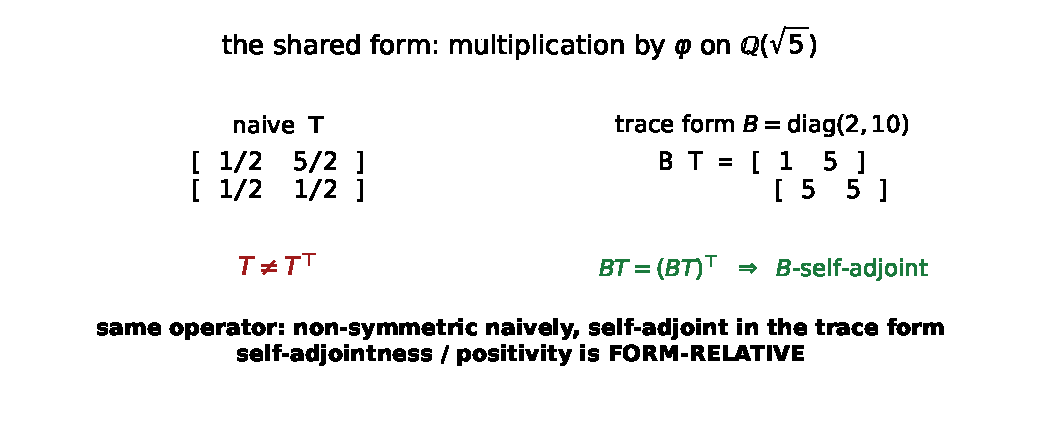
\includegraphics[width=0.96\linewidth]{fig_form_relativity.pdf}
\caption{Form-relativity (exact). The multiplication-by-$\varphi$ operator is not symmetric
under the naive form but is self-adjoint under the trace form $B$; equivalently the
$H_4\to E_8$ inner-product residual closes from $\pm\tfrac12$ to $0$.}\label{fig:formrel}
\end{figure}

\section{Instance G --- geometry: the form delivers closure (exact)}\label{sec:geom}
The icosian/$H_4$ data embeds into $E_8$ only after the naive map $x\mapsto(x,\sigma x)$
(inner products $\pm\tfrac12$, not even-integral) is completed to the \emph{golden trace
form} $B(x,y)=\Tr_{\Q(\sqrt5)/\Q}\!\bigl(c\,\langle x,y\rangle\bigr)$ with $c=1+1/\sqrt5$
(so $\Tr c=2$), \emph{derived} by the norm-$2$ and integrality constraints. Under $B$,
\[
  \text{shell}_1\ \cup\ (1/\varphi)\,\text{shell}_1\ =\ 240\ \text{roots},\quad
  \|\cdot\|^2=2,\quad \text{root graph }(56,56,126,1,1),\ \text{rank }8,\ \text{even integral},
\]
i.e.\ the canonical $E_8$ (Fig.~\ref{fig:e8}). The residual closes $\pm\tfrac12\to0$:
\emph{the form delivers closure, exactly}. This is the known Wilson / Moody--Patera
construction \cite{Wilson,MoodyPatera}, verified; we use it as the one instance where
Principle~\ref{prin:main} is \emph{realised}, not merely posited.

\begin{figure}[t]\centering
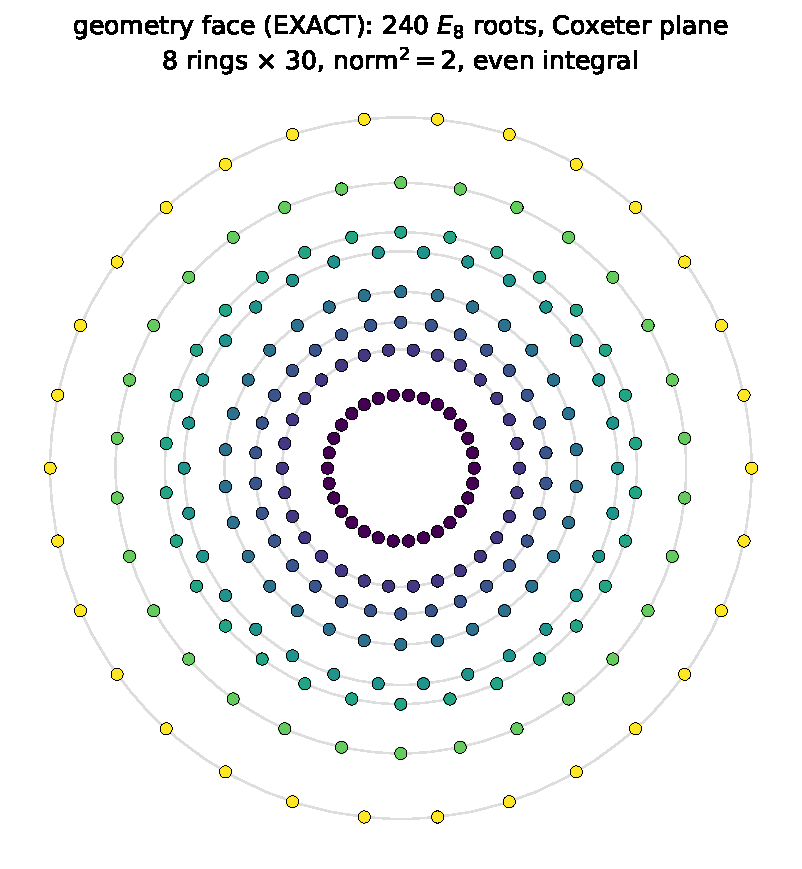
\includegraphics[width=0.52\linewidth]{fig_e8_coxeter.pdf}
\caption{Instance G (\textsc{exact}). The $240$ $E_8$ roots, $\text{shell}_1\cup
(1/\varphi)\text{shell}_1$, in the Coxeter plane: eight concentric rings of $30$ (verified
$240=8\times30$). Under the golden trace form the structure is even-integral $E_8$ --- the
form closes it.}\label{fig:e8}
\end{figure}

\section{Instance A --- arithmetic: the form is known, closure is RH (open)}\label{sec:arith}
The same pattern, on the scale axis. For the self-dual cuspidal $L$-function $L(s,\pi)$ of
the icosian Brandt face at level $\mathfrak p_{31}$ over $K=\Q(\sqrt5)$, the naive prime-only
kernel is non-positive and divergent; completing to the Weil/Connes form --- archimedean
boundary $A_\infty$ (gamma factor, from Tate's local theory on the scale axis) minus the
geometric prime residue $A_P$ (scale-translations weighted by the icosian Brandt eigenvalues
$a_\fq$) --- yields a self-adjoint operator
\[
  A=A_\infty-A_P,\qquad \langle h,Ah\rangle=\sum_\rho|\widehat h(\gamma_\rho)|^2,\qquad
  \boxed{\,A\ge0\iff \text{RH}(L)\,}
\]
(the identification lemma and the equivalence are established in the companion
\cite{Witness}; Fig.~\ref{fig:witness}). Here the canonical form is the explicit formula
itself, and it is \emph{finite-positive} on every tested band --- yet \textbf{full positivity
is exactly RH$(L)$, and is open}. This is the standing counterexample to a guarantee: the
right form is present and finite-positive, and closure is still not delivered. (Scope: RH$(L)$
is GRH for this one cuspidal $L$, \emph{not} classical $\zeta$; no RH proof is claimed.)

\begin{figure}[t]\centering
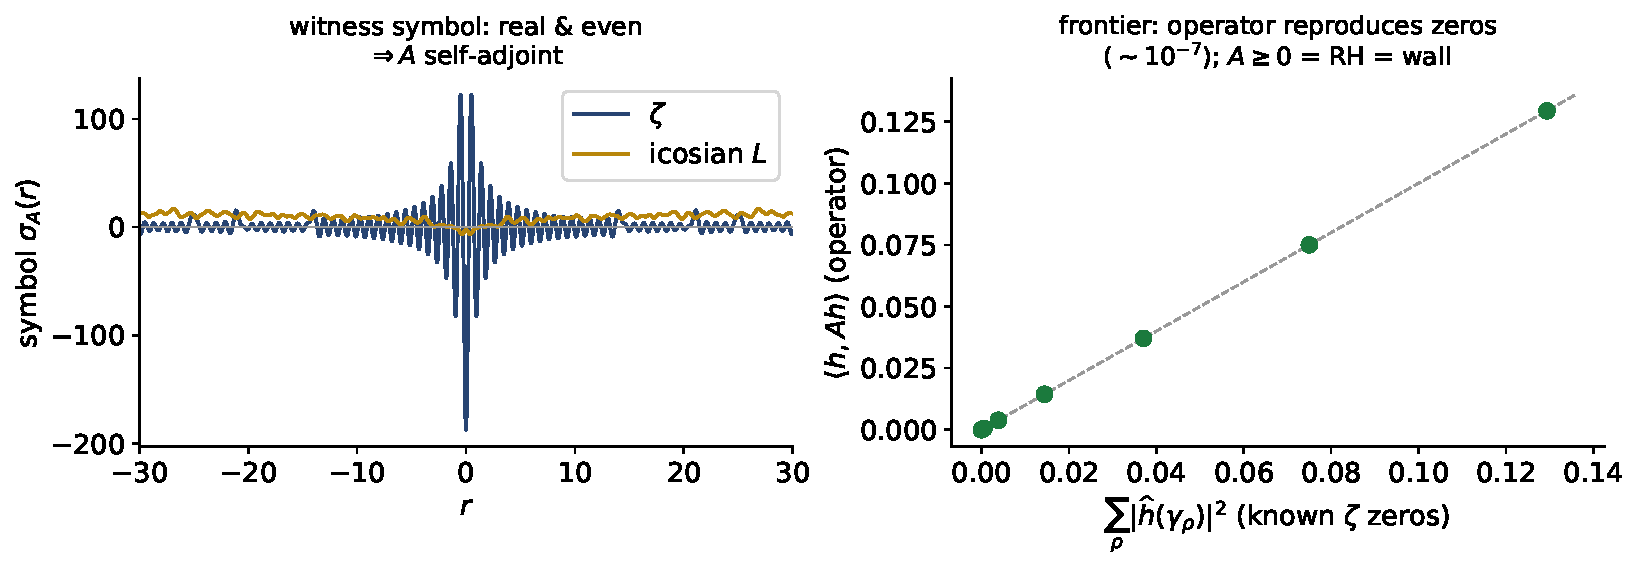
\includegraphics[width=0.96\linewidth]{fig_witness_symbol.pdf}
\caption{Instance A (\textsc{open}). Left: the witness-operator symbol $\sigma_A(r)=
\omega_\infty-\widehat{A_P}$ for $\zeta$ and for the icosian $L$ --- real and even, so $A$
is self-adjoint. Right: the operator form reproduces the sum over the known Riemann zeros to
$\sim10^{-7}$ (the identification lemma). Positivity of $A$ for \emph{all} $h$ is the wall =
RH$(L)$; it is not shown.}\label{fig:witness}
\end{figure}

\section{Instance P --- physics: shared architecture, no transfer (analogy)}\label{sec:phys}
A third appearance is dynamical. A static ``funnel'' geometry is cosmetic (the radius is a
bijection, no invariant); completing to the \emph{scattering determinant} / Jost function
with a greybody ($\Gamma$-ratio) factor produces a genuine architecture --- determinant
$\to$ log-derivative (digamma) $\to$ resonances on lines $\to$ stability --- the known
trace-formula / Lax--Phillips picture. For a \emph{real} (self-adjoint) potential this gives
damped quasinormal modes; but the arithmetic instance of the \emph{same} statement is
Hilbert--P\'olya, i.e.\ RH. So the form/architecture is \emph{parallel}, and the closure does
\emph{not} transfer: the toy is provable because its potential is self-adjoint; the
arithmetic self-adjointness is open. This instance is \textbf{analogy only}. (The
$\sigma$-paired closure form also appears in a separate cosmological \emph{model}
\cite{Cosmo}; that is a physical model on the same geometry, firewalled from the arithmetic
--- see \S\ref{sec:unif}.)

\section{The unification: one principle, three forms, no implication}\label{sec:unif}
\begin{figure}[t]\centering
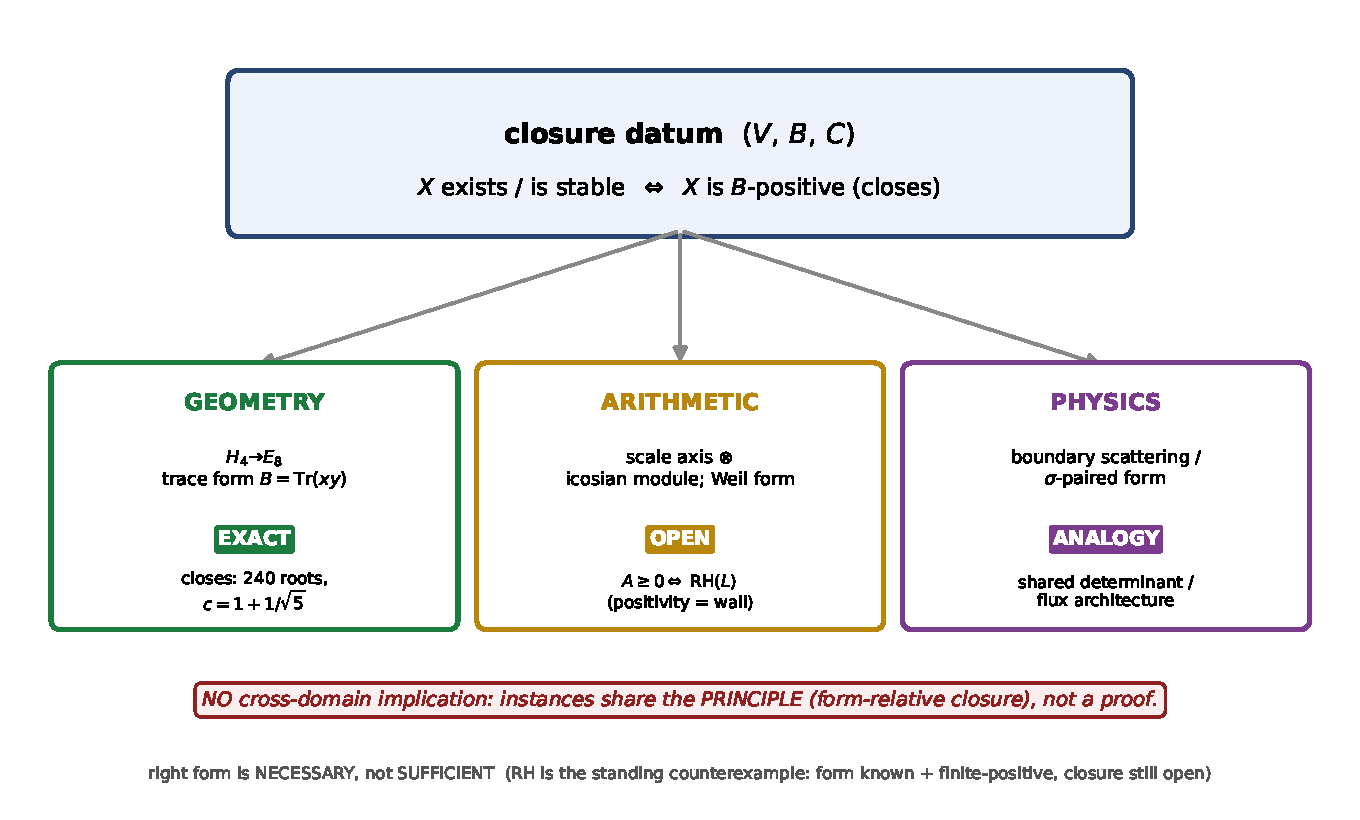
\includegraphics[width=0.96\linewidth]{fig_unification_map.pdf}
\caption{The map. One closure datum; three graded instances. Geometry: the form delivers
closure (exact). Arithmetic: the form is known, closure is RH (open). Physics: shared
architecture, analogy only. The instances share the \emph{principle}, not a proof: there is
no cross-domain implication, and the right form is necessary, not sufficient.}\label{fig:map}
\end{figure}

Putting the instances on one map (Fig.~\ref{fig:map}):
\begin{center}\small
\begin{tabular}{llll}
\hline
instance & closure datum $(V,B)$ & ``closes'' means & status \\
\hline
geometry & $H_4$ data, golden trace form & even-integral $E_8$ (240 roots) & \textsc{exact} (proved) \\
arithmetic & scale axis $\otimes$ icosian module, Weil form & $A\ge0\iff$ RH$(L)$ & \textsc{open} (positivity = RH) \\
physics & boundary geometry, scattering/$\sigma$ form & self-adjoint $\Rightarrow$ stable modes & \textsc{analogy} (no transfer) \\
\hline
\end{tabular}
\end{center}

\noindent\textbf{What relates them.} The shared object is the closure datum and
Principle~\ref{prin:main}: in each domain, \emph{exists/stable $\iff$ $B$-positive}. The
relation lives at the level of the abstract datum $(V,B,C)$, realised independently in each
domain; the recurring concrete structures ($E_8/H_4$, $\sigma$-pairing, the closure operator)
are a shared \emph{vocabulary}.

\noindent\textbf{What does not relate them (firewall).} There is \emph{no} implication
geometry $\Rightarrow$ arithmetic $\Rightarrow$ physics. The geometry does not prove the
arithmetic; no physical model implies or is implied by $\zeta$. Each instance has its own,
independent status. This is deliberate and load-bearing: because no instance props up
another, no instance can drag another down. The proved geometric instance shows the
principle is \emph{not vacuous}; the arithmetic instance gives it a precise equivalent of RH;
the physical instance shows reach. One proved, one equivalence, one analogy.

\section{The object behind the scale axis}\label{sec:object}
The arithmetic instance lives on a scale axis whose two ends and equator are one
compactified object $\mathcal{V}_1=([-\infty,+\infty]\times S^1,\pi,Q)$, $\pi(t,\theta)=
e^{t/2}e^{i\theta}$: the point ($t\to-\infty$), the unit circle ($t=0$, read as the critical
line), and infinity ($t\to+\infty$) are three boundary cuts of one object, with the mirror
$t\mapsto-t$ the functional equation and the closure law $Q[\Phi]\ge0$ the positivity
(Fig.~\ref{fig:cyl}). This is the interpretive picture that motivates the arithmetic instance;
it is not load-bearing for any theorem here.

\begin{figure}[t]\centering
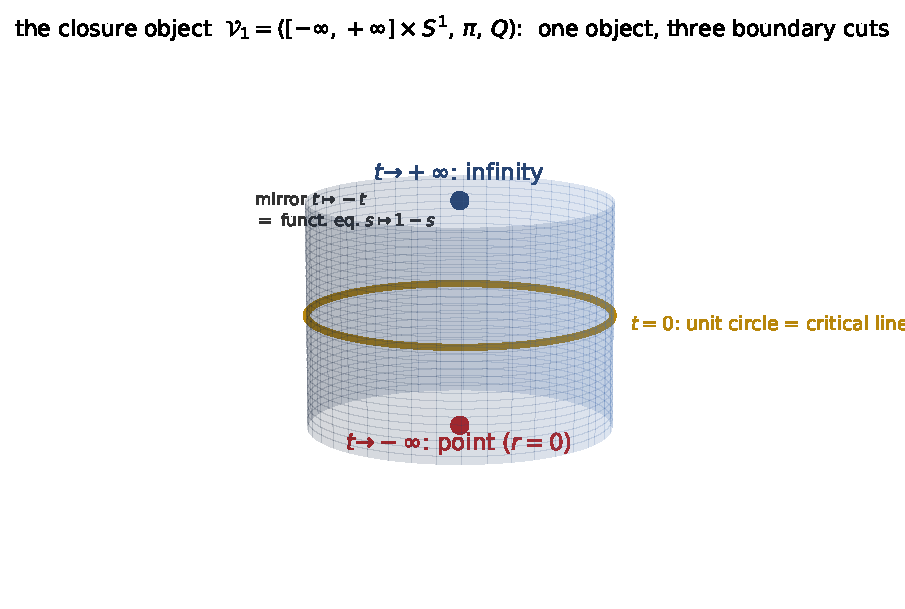
\includegraphics[width=0.78\linewidth]{fig_cylinder.pdf}
\caption{The closure object $\mathcal{V}_1$ (interpretation). One compactified scale--phase
object; point, equator (critical line), and infinity are its three boundary cuts; the
closure law is $Q[\Phi]\ge0$.}\label{fig:cyl}
\end{figure}

\section{Scope}\label{sec:scope}
We state a form-relativity lens (Lemma~\ref{lem:formrel}, exact), one proved instance where
the form delivers closure ($H_4\to E_8$), one instance where the canonical form is known and
finite-positive yet closure is RH (open), and one analogy (scattering). We do \emph{not}
prove RH; we do \emph{not} claim the principle forces closure (RH refutes the guarantee
version); we do \emph{not} claim any cross-domain implication, nor any connection between a
physical model and $\zeta$. The unification is the principle with its instances --- a lens
and a search heuristic, with one exact exemplar --- not a theorem that unifies by proof.

\begin{thebibliography}{9}
\bibitem{Wilson} R.~A.~Wilson, \emph{The geometry of the Hall--Janko group as a quaternionic
  reflection group}, and related icosian/$E_8$ constructions.
\bibitem{MoodyPatera} R.~V.~Moody and J.~Patera, \emph{Quasicrystals and icosians},
  J.~Phys.~A \textbf{26} (1993).
\bibitem{Witness} VFD programme, \emph{A Witness Operator on the Scale Axis} (companion
  draft): $A=A_\infty-A_P$, $\langle h,Ah\rangle=\sum_\rho|\widehat h(\gamma_\rho)|^2$,
  $A\ge0\iff$ RH$(L)$; geometric Brandt coefficients; numerical corroboration.
\bibitem{Cosmo} VFD programme, \emph{Hypersphere Cosmology} (v1.1): the $\sigma$-paired
  dipole closure as a cosmological model (separate domain; firewalled from RH).
\bibitem{Connes} A.~Connes, \emph{Trace formula in noncommutative geometry and the zeros of
  the Riemann zeta function}, Selecta Math.\ (1999).
\bibitem{Weil} A.~Weil, \emph{Sur les ``formules explicites''\ldots}; the explicit formula
  and the positivity criterion.
\bibitem{TFL} VFD programme, \emph{Invariant Trace-Form Closure} (internal report
  WO-VFD-INVARIANT-TRACE-FORM-LAW-001): the three-case grading this paper formalises.
\end{thebibliography}

\end{document}
